%!TEX root = ./main.tex

Denotemos $\mathcal{B}_n$ como el conjunto de trenzas en $n$ cuerdas con la multiplicacion dada en la Definicion 2.6, veamos que efectivamente es un grupo
\begin{prop}
    $\mathcal{B}_n$ es un grupo.
\end{prop}
\begin{proof}
    Previamente ya habíamos visto que con esta operación el conjunto es un monoide, nos bastaría encontrar un inverso para cada $\beta\in \mathcal{B}_n$. Para $i=1,\ldots,n-1$, definimos $\sigma_i^+$ y $\sigma_i^-$ dadas en la siguiente figura
    \begin{center}
        
    

\tikzset{every picture/.style={line width=0.75pt}} %set default line width to 0.75pt        

\begin{tikzpicture}[x=0.75pt,y=0.75pt,yscale=-1.5,xscale=1.5]
%uncomment if require: \path (0,300); %set diagram left start at 0, and has height of 300

%Straight Lines [id:da43485227266233983] 
\draw    (170,20) -- (170,120) ;
%Straight Lines [id:da9331696760365621] 
\draw    (210,20) -- (210,120) ;
%Straight Lines [id:da9617020865382828] 
\draw    (300,20) -- (300,120) ;
%Straight Lines [id:da23545398468453227] 
\draw    (340,20) -- (340,120) ;
%Curve Lines [id:da7964129888127446] 
\draw    (240,120) .. controls (240.6,69.8) and (269.8,69.8) .. (270,20) ;
%Curve Lines [id:da9092522991774518] 
\draw    (240,20) .. controls (242.2,52.6) and (244.6,60.6) .. (251,67) ;
%Curve Lines [id:da14137481359772275] 
\draw    (259,73) .. controls (263.6,82.6) and (270.2,92.6) .. (270,120) ;
%Straight Lines [id:da7700112899007484] 
\draw    (170,149) -- (170,249) ;
%Straight Lines [id:da5513354586153557] 
\draw    (210,149) -- (210,249) ;
%Straight Lines [id:da6374072931177768] 
\draw    (300,149) -- (300,249) ;
%Straight Lines [id:da704810691253697] 
\draw    (340,149) -- (340,249) ;
%Curve Lines [id:da20368613461263263] 
\draw    (270,249) .. controls (270.6,198.8) and (239.8,199.8) .. (240,150) ;
%Curve Lines [id:da48874246949849454] 
\draw    (270,150) .. controls (270.2,182.6) and (262.4,187.2) .. (257,195) ;
%Curve Lines [id:da2656325163455132] 
\draw    (251,200) .. controls (243.2,207) and (240.2,222.6) .. (240,250) ;

% Text Node
\draw (176,59.4) node [anchor=north west][inner sep=0.75pt]    {$\cdots $};
% Text Node
\draw (306,60.4) node [anchor=north west][inner sep=0.75pt]    {$\cdots $};
% Text Node
\draw (166,5.4) node [anchor=north west][inner sep=0.75pt]  [font=\scriptsize]  {$1$};
% Text Node
\draw (199,6.4) node [anchor=north west][inner sep=0.75pt]  [font=\scriptsize]  {$i-1$};
% Text Node
\draw (237,6.4) node [anchor=north west][inner sep=0.75pt]  [font=\scriptsize]  {$i$};
% Text Node
\draw (259,6.4) node [anchor=north west][inner sep=0.75pt]  [font=\scriptsize]  {$i+1$};
% Text Node
\draw (289,6.4) node [anchor=north west][inner sep=0.75pt]  [font=\scriptsize]  {$i+2$};
% Text Node
\draw (336,5.4) node [anchor=north west][inner sep=0.75pt]  [font=\scriptsize]  {$n$};
% Text Node
\draw (138,56.4) node [anchor=north west][inner sep=0.75pt]    {$\sigma _{i}^{+}$};
% Text Node
\draw (176,188.4) node [anchor=north west][inner sep=0.75pt]    {$\cdots $};
% Text Node
\draw (306,189.4) node [anchor=north west][inner sep=0.75pt]    {$\cdots $};
% Text Node
\draw (166,134.4) node [anchor=north west][inner sep=0.75pt]  [font=\scriptsize]  {$1$};
% Text Node
\draw (199,135.4) node [anchor=north west][inner sep=0.75pt]  [font=\scriptsize]  {$i-1$};
% Text Node
\draw (237,135.4) node [anchor=north west][inner sep=0.75pt]  [font=\scriptsize]  {$i$};
% Text Node
\draw (259,135.4) node [anchor=north west][inner sep=0.75pt]  [font=\scriptsize]  {$i+1$};
% Text Node
\draw (289,135.4) node [anchor=north west][inner sep=0.75pt]  [font=\scriptsize]  {$i+2$};
% Text Node
\draw (336,134.4) node [anchor=north west][inner sep=0.75pt]  [font=\scriptsize]  {$n$};
% Text Node
\draw (138,185.4) node [anchor=north west][inner sep=0.75pt]    {$\sigma _{i}^{-}$};


\end{tikzpicture}

    \end{center}
    Veamos que el conjunto de todas estas genera a cualquier trenza $\beta\in \mathcal{B}_n$. consideremos el diagrama de trenzas $D\subset\R\times I$ que la representa. Como hay una cantidad finita $k$ de intersecciones en el diagrama podemos deformarlo de tal manera que cada intersección se de en una segunda coordenada diferente, es decir podemos conseguir una partición del intervalo
    $$0=t_0<t_1<\dots<t_{k-1}<t_k=1,$$
    tal que cada banda $\R\times[t_j,t_{j+1}]$ posee exactamente una intersección en el interior de cada banda. Así cada una de estas bandas se puede ver como una reparametrizacion de la trenza $\sigma_i^+$ o $\sigma_i^-$, así con el producto obtenemos que
    $$\beta=\beta(D)=\sigma_{i_1}^{\varepsilon_1}\dots\sigma_{i_k}^{\varepsilon_k},$$
    donde cada $\varepsilon_j=\pm$ y $i_j\in\{1,2,\ldots,n-1\}$.
    Así como cada $\sigma_i^+\sigma_i^-=\sigma_i^-\sigma_i^+=1$, debido a que este diagrama es equivalente al trivial aplicando $\Omega_2$. Así el elemento inverso es
    $$\beta^{-1}=\sigma_{i_k}^{-\varepsilon_k}\dots\sigma_{i_1}^{-\varepsilon_1}.$$ 
    Mostrando así que es un grupo. 
\end{proof}
\begin{eg}
    Para ver esta idea en acción en el siguiente diagrama podemos ver una trenza de $\mathcal{B}_3$ su inverso y el proceso de usar consecutivamente $\Omega_2$ para convertir la concatenación en $1_3$
    \begin{center}
        

\tikzset{every picture/.style={line width=0.75pt}} %set default line width to 0.75pt        

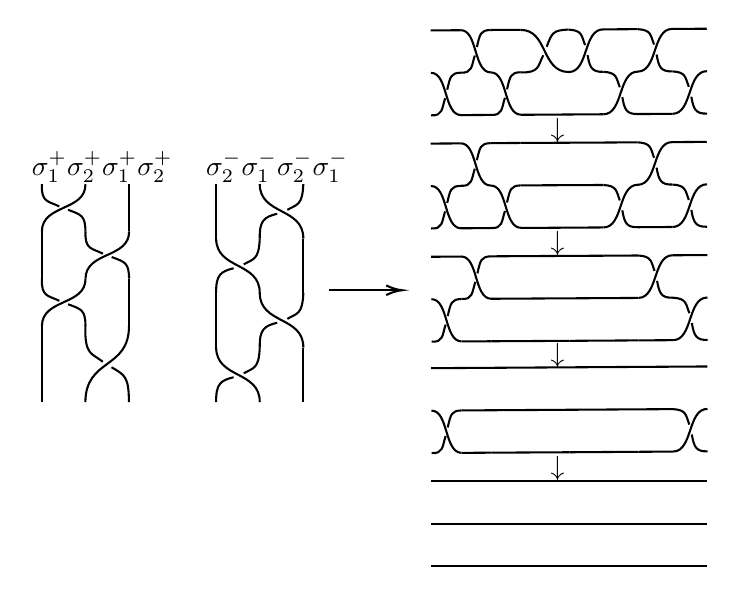
\begin{tikzpicture}[x=0.75pt,y=0.75pt,yscale=-0.7,xscale=0.7]
%uncomment if require: \path (0,877); %set diagram left start at 0, and has height of 877

%Curve Lines [id:da427260159128515] 
\draw    (62.05,127) .. controls (62.25,145.66) and (32.25,140.65) .. (32.05,159.5) ;
%Straight Lines [id:da669144458368129] 
\draw    (92.05,127) -- (92.05,159.5) ;
%Curve Lines [id:da5875226797100279] 
\draw    (32.05,127) .. controls (31.45,139.72) and (36.65,138.61) .. (44.05,142.32) ;
%Curve Lines [id:da8023235603797557] 
\draw    (50.05,144.64) .. controls (59.45,148.08) and (61.85,148.64) .. (62.05,159.5) ;
%Curve Lines [id:da9691807928909935] 
\draw    (92.09,159.5) .. controls (92.29,178.16) and (62.29,173.15) .. (62.09,192) ;
%Straight Lines [id:da8189246846133199] 
\draw    (32.05,159.5) -- (32.05,192) ;
%Curve Lines [id:da03334011193119202] 
\draw    (62.09,159.5) .. controls (61.49,172.22) and (66.69,171.11) .. (74.09,174.82) ;
%Curve Lines [id:da9703929579231297] 
\draw    (80.09,177.14) .. controls (89.49,180.58) and (91.89,181.14) .. (92.09,192) ;
%Curve Lines [id:da3476578065648639] 
\draw    (62.09,192) .. controls (62.29,210.66) and (32.29,205.65) .. (32.09,224.5) ;
%Straight Lines [id:da6047039693312939] 
\draw    (92.09,192) -- (92.09,224.5) ;
%Curve Lines [id:da9132235245863184] 
\draw    (32.09,192) .. controls (31.49,204.72) and (36.69,203.61) .. (44.09,207.32) ;
%Curve Lines [id:da7963348295748283] 
\draw    (50.09,209.64) .. controls (59.49,213.08) and (61.89,213.64) .. (62.09,224.5) ;
%Curve Lines [id:da11214896674466468] 
\draw    (92,224.5) .. controls (92.2,254.65) and (62.2,246.55) .. (62,277) ;
%Straight Lines [id:da5785722857796761] 
\draw    (32,224.5) -- (32,277) ;
%Curve Lines [id:da4563642723889444] 
\draw    (62,224.5) .. controls (61.4,245.05) and (66.6,243.25) .. (74,249.25) ;
%Curve Lines [id:da011566386673468099] 
\draw    (80,253) .. controls (89.4,258.55) and (91.8,259.45) .. (92,277) ;
%Curve Lines [id:da9127778046127226] 
\draw    (182,127) .. controls (182.2,148.54) and (212.2,142.75) .. (212,164.5) ;
%Straight Lines [id:da008174707632187195] 
\draw    (152,127) -- (152,164.5) ;
%Curve Lines [id:da45462127023717136] 
\draw    (212,127) .. controls (211.4,141.68) and (207.8,140.82) .. (201,144.68) ;
%Curve Lines [id:da9247943883726462] 
\draw    (194,147.36) .. controls (185,149.61) and (181.8,151.96) .. (182,164.5) ;
%Curve Lines [id:da304291960900533] 
\draw    (152.01,164.5) .. controls (152.21,186.04) and (182.21,180.25) .. (182.01,202) ;
%Straight Lines [id:da9527368578332924] 
\draw    (212.01,164.5) -- (212.01,202) ;
%Curve Lines [id:da12684543359533484] 
\draw    (182.01,164.5) .. controls (181.41,179.18) and (177.81,178.32) .. (171.01,182.18) ;
%Curve Lines [id:da6114193569445832] 
\draw    (164.01,184.86) .. controls (155.01,187.11) and (151.81,189.46) .. (152.01,202) ;
%Curve Lines [id:da010831733150057254] 
\draw    (182.01,202) .. controls (182.21,223.54) and (212.21,217.75) .. (212.01,239.5) ;
%Straight Lines [id:da03536115402034823] 
\draw    (152,202) -- (152,239.5) ;
%Curve Lines [id:da6439072709175471] 
\draw    (212.01,202) .. controls (211.41,216.68) and (207.81,215.82) .. (201.01,219.68) ;
%Curve Lines [id:da23875994271201506] 
\draw    (194.01,222.36) .. controls (185.01,224.61) and (181.81,226.96) .. (182.01,239.5) ;
%Curve Lines [id:da8697709322375486] 
\draw    (152.01,239.5) .. controls (152.21,261.04) and (182.21,255.25) .. (182.01,277) ;
%Straight Lines [id:da6076361908657307] 
\draw    (212.01,239.5) -- (212.01,277) ;
%Curve Lines [id:da47015848638541236] 
\draw    (182.01,239.5) .. controls (181.41,254.18) and (177.81,253.32) .. (171.01,257.18) ;
%Curve Lines [id:da3578205966770538] 
\draw    (164.01,259.86) .. controls (155.01,262.11) and (151.81,264.46) .. (152.01,277) ;
%Curve Lines [id:da531599854802458] 
\draw    (299.81,50.39) .. controls (311.63,50.12) and (308.61,79.35) .. (320.56,79.46) ;
%Straight Lines [id:da7115570026778073] 
\draw    (299.65,21.18) -- (320.23,21.04) ;
%Curve Lines [id:da20874798824463314] 
\draw    (299.97,79.6) .. controls (308.03,80.13) and (307.3,75.07) .. (309.61,67.85) ;
%Curve Lines [id:da16452737584436772] 
\draw    (311.05,62) .. controls (313.17,52.83) and (313.51,50.49) .. (320.4,50.25) ;
%Curve Lines [id:da0001267340971137232] 
\draw    (320.23,21) .. controls (332.06,20.73) and (329.04,49.96) .. (340.98,50.08) ;
%Straight Lines [id:da7580512650775525] 
\draw    (320.56,79.46) -- (341.14,79.33) ;
%Curve Lines [id:da9957192227611716] 
\draw    (320.39,50.21) .. controls (328.46,50.74) and (327.72,45.68) .. (330.04,38.46) ;
%Curve Lines [id:da2752293919286407] 
\draw    (331.47,32.61) .. controls (333.6,23.45) and (333.94,21.11) .. (340.82,20.87) ;
%Curve Lines [id:da4248810803242654] 
\draw    (340.98,50.08) .. controls (352.8,49.81) and (349.79,79.04) .. (361.73,79.16) ;
%Straight Lines [id:da8504788815198621] 
\draw    (340.82,20.87) -- (361.41,20.74) ;
%Curve Lines [id:da9144139734174279] 
\draw    (341.14,79.29) .. controls (349.2,79.82) and (348.47,74.76) .. (350.78,67.54) ;
%Curve Lines [id:da5788507049444858] 
\draw    (352.22,61.69) .. controls (354.35,52.52) and (354.69,50.18) .. (361.57,49.95) ;
%Curve Lines [id:da24991551123604183] 
\draw    (361.41,20.83) .. controls (380.5,20.51) and (375.53,49.75) .. (394.82,49.83) ;
%Straight Lines [id:da2279207192126409] 
\draw    (361.73,79.25) -- (394.98,79.04) ;
%Curve Lines [id:da869940382936184] 
\draw    (361.57,50.04) .. controls (374.59,50.54) and (373.42,45.48) .. (377.18,38.25) ;
%Curve Lines [id:da4641619409636202] 
\draw    (379.52,32.4) .. controls (382.99,23.22) and (383.55,20.88) .. (394.66,20.62) ;
%Curve Lines [id:da9490813438634549] 
\draw    (394.82,49.83) .. controls (408.46,49.54) and (404.64,20.36) .. (418.42,20.46) ;
%Straight Lines [id:da68328132238534] 
\draw    (394.98,79.04) -- (418.74,78.88) ;
%Curve Lines [id:da12353792960760934] 
\draw    (394.66,20.62) .. controls (403.96,21.14) and (403.44,24.65) .. (405.92,31.26) ;
%Curve Lines [id:da6705891019087905] 
\draw    (407.65,38.06) .. controls (409.13,46.81) and (410.64,49.92) .. (418.58,49.67) ;
%Curve Lines [id:da9239147121814012] 
\draw    (418.74,78.88) .. controls (432.38,78.59) and (428.55,49.41) .. (442.33,49.51) ;
%Straight Lines [id:da18931787803211197] 
\draw    (418.42,20.46) -- (442.17,20.3) ;
%Curve Lines [id:da29055757381703284] 
\draw    (418.58,49.67) .. controls (427.88,50.19) and (427.36,53.7) .. (429.83,60.3) ;
%Curve Lines [id:da5425206352743233] 
\draw    (431.57,67.11) .. controls (433.04,75.86) and (434.55,78.97) .. (442.49,78.72) ;
%Curve Lines [id:da41494150959375964] 
\draw    (442.33,49.51) .. controls (455.97,49.23) and (452.15,20.04) .. (465.92,20.15) ;
%Straight Lines [id:da132979245306439] 
\draw    (442.49,78.73) -- (466.25,78.58) ;
%Curve Lines [id:da5680042325328389] 
\draw    (442.17,20.3) .. controls (451.47,20.83) and (450.95,24.34) .. (453.43,30.94) ;
%Curve Lines [id:da6672133326873362] 
\draw    (455.16,37.75) .. controls (456.64,46.5) and (458.15,49.61) .. (466.09,49.36) ;
%Curve Lines [id:da5764858313819528] 
\draw    (466.25,78.57) .. controls (479.89,78.29) and (476.06,49.1) .. (489.84,49.21) ;
%Straight Lines [id:da9437582235565463] 
\draw    (465.92,20.15) -- (489.68,20) ;
%Curve Lines [id:da3423748266275308] 
\draw    (466.09,49.36) .. controls (475.39,49.89) and (474.86,53.4) .. (477.34,60) ;
%Curve Lines [id:da20080394546758273] 
\draw    (479.08,66.81) .. controls (480.55,75.56) and (482.06,78.67) .. (490,78.42) ;
%Straight Lines [id:da9678508680287174] 
\draw    (230,200) -- (278,200) ;
\draw [shift={(280,200)}, rotate = 180] [color={rgb, 255:red, 0; green, 0; blue, 0 }  ][line width=0.75]    (10.93,-3.29) .. controls (6.95,-1.4) and (3.31,-0.3) .. (0,0) .. controls (3.31,0.3) and (6.95,1.4) .. (10.93,3.29)   ;
%Curve Lines [id:da7308439505195594] 
\draw    (299.81,128.28) .. controls (311.63,128.01) and (308.61,157.24) .. (320.56,157.36) ;
%Straight Lines [id:da846513170034754] 
\draw    (299.65,99.07) -- (320.23,98.94) ;
%Curve Lines [id:da8111277427735796] 
\draw    (299.97,157.49) .. controls (308.03,158.02) and (307.3,152.97) .. (309.61,145.74) ;
%Curve Lines [id:da42089992613742544] 
\draw    (311.05,139.89) .. controls (313.17,130.73) and (313.51,128.39) .. (320.4,128.15) ;
%Curve Lines [id:da8563546535375895] 
\draw    (320.23,98.89) .. controls (332.06,98.62) and (329.04,127.85) .. (340.98,127.97) ;
%Straight Lines [id:da4667452310801803] 
\draw    (320.56,157.36) -- (341.14,157.23) ;
%Curve Lines [id:da40900442234538137] 
\draw    (320.39,128.1) .. controls (328.46,128.64) and (327.72,123.58) .. (330.04,116.36) ;
%Curve Lines [id:da2505747526551777] 
\draw    (331.47,110.51) .. controls (333.6,101.34) and (333.94,99) .. (340.82,98.76) ;
%Curve Lines [id:da1318615718347721] 
\draw    (340.98,127.97) .. controls (352.8,127.7) and (349.79,156.93) .. (361.73,157.05) ;
%Straight Lines [id:da33122994992169363] 
\draw    (340.82,98.76) -- (361.41,98.63) ;
%Curve Lines [id:da4392684723589957] 
\draw    (341.14,157.18) .. controls (349.2,157.71) and (348.47,152.66) .. (350.78,145.44) ;
%Curve Lines [id:da14605677214321222] 
\draw    (352.22,139.58) .. controls (354.35,130.42) and (354.69,128.08) .. (361.57,127.84) ;
%Straight Lines [id:da3422396945440085] 
\draw    (361.73,157.14) -- (394.98,156.93) ;
%Straight Lines [id:da5773890702994031] 
\draw    (394.98,156.93) -- (418.74,156.78) ;
%Curve Lines [id:da9252240206443388] 
\draw    (418.74,156.77) .. controls (432.38,156.49) and (428.55,127.3) .. (442.33,127.41) ;
%Straight Lines [id:da08142014538727405] 
\draw    (418.42,98.35) -- (442.17,98.2) ;
%Curve Lines [id:da6043299896294531] 
\draw    (418.58,127.56) .. controls (427.88,128.08) and (427.36,131.59) .. (429.83,138.2) ;
%Curve Lines [id:da857933680416637] 
\draw    (431.57,145) .. controls (433.04,153.76) and (434.55,156.86) .. (442.49,156.62) ;
%Curve Lines [id:da558444715983223] 
\draw    (442.33,127.41) .. controls (455.97,127.13) and (452.15,97.94) .. (465.92,98.05) ;
%Straight Lines [id:da0010087886285466974] 
\draw    (442.49,156.63) -- (466.25,156.47) ;
%Curve Lines [id:da6558981134377307] 
\draw    (442.17,98.2) .. controls (451.47,98.72) and (450.95,102.23) .. (453.43,108.84) ;
%Curve Lines [id:da20262856244113558] 
\draw    (455.16,115.64) .. controls (456.64,124.4) and (458.15,127.5) .. (466.09,127.26) ;
%Curve Lines [id:da9402828684572856] 
\draw    (466.25,156.47) .. controls (479.89,156.18) and (476.06,127) .. (489.84,127.1) ;
%Straight Lines [id:da0655025037371203] 
\draw    (465.92,98.05) -- (489.68,97.89) ;
%Curve Lines [id:da276379066843348] 
\draw    (466.09,127.26) .. controls (475.39,127.78) and (474.86,131.29) .. (477.34,137.9) ;
%Curve Lines [id:da02073947493596051] 
\draw    (479.08,144.7) .. controls (480.55,153.45) and (482.06,156.56) .. (490,156.31) ;
%Straight Lines [id:da7950315894943095] 
\draw    (361.41,98.63) -- (418.42,98.35) ;
%Straight Lines [id:da45172338628325837] 
\draw    (361.57,127.84) -- (418.58,127.56) ;
%Curve Lines [id:da8320898145842732] 
\draw    (300.16,206.18) .. controls (311.98,205.91) and (308.97,235.14) .. (320.91,235.25) ;
%Straight Lines [id:da2548387102144052] 
\draw    (300,176.97) -- (320.59,176.83) ;
%Curve Lines [id:da409883616871649] 
\draw    (300.32,235.39) .. controls (308.38,235.92) and (307.65,230.86) .. (309.96,223.64) ;
%Curve Lines [id:da8710039812889714] 
\draw    (311.4,217.79) .. controls (313.53,208.62) and (313.87,206.28) .. (320.75,206.04) ;
%Curve Lines [id:da4884793512039546] 
\draw    (320.59,176.79) .. controls (332.41,176.52) and (329.39,205.75) .. (341.33,205.87) ;
%Straight Lines [id:da4873947944494157] 
\draw    (320.91,235.25) -- (341.5,235.12) ;
%Curve Lines [id:da13237144060625328] 
\draw    (320.75,206) .. controls (328.81,206.53) and (328.08,201.47) .. (330.39,194.25) ;
%Curve Lines [id:da5907249199798268] 
\draw    (331.83,188.4) .. controls (333.95,179.23) and (334.29,176.9) .. (341.17,176.66) ;
%Straight Lines [id:da14164508530301012] 
\draw    (341.17,176.66) -- (361.76,176.53) ;
%Straight Lines [id:da8889099653035093] 
\draw    (341.5,235.12) -- (395.34,234.82) ;
%Straight Lines [id:da8237680629290057] 
\draw    (395.34,234.82) -- (442.85,234.52) ;
%Straight Lines [id:da5430475777888927] 
\draw    (418.77,176.24) -- (442.52,176.09) ;
%Curve Lines [id:da48506072461021554] 
\draw    (442.68,205.3) .. controls (456.32,205.02) and (452.5,175.83) .. (466.28,175.94) ;
%Straight Lines [id:da5608790679234237] 
\draw    (442.85,234.52) -- (466.6,234.37) ;
%Curve Lines [id:da894534360023443] 
\draw    (442.52,176.09) .. controls (451.82,176.62) and (451.3,180.13) .. (453.78,186.73) ;
%Curve Lines [id:da30195238061608853] 
\draw    (455.51,193.54) .. controls (456.99,202.29) and (458.5,205.4) .. (466.44,205.15) ;
%Curve Lines [id:da34717666389077595] 
\draw    (466.6,234.36) .. controls (480.24,234.08) and (476.41,204.89) .. (490.19,205) ;
%Straight Lines [id:da5707306301760324] 
\draw    (466.28,175.94) -- (490.03,175.79) ;
%Curve Lines [id:da39489551630013087] 
\draw    (466.44,205.15) .. controls (475.74,205.68) and (475.22,209.18) .. (477.69,215.79) ;
%Curve Lines [id:da32809801630168434] 
\draw    (479.43,222.59) .. controls (480.9,231.35) and (482.41,234.45) .. (490.35,234.21) ;
%Straight Lines [id:da78774750197805] 
\draw    (361.76,176.53) -- (418.77,176.24) ;
%Straight Lines [id:da5555019473591153] 
\draw    (341.33,205.87) -- (442.68,205.3) ;
%Curve Lines [id:da10634566902173404] 
\draw    (300.16,282.86) .. controls (311.98,282.59) and (308.97,311.82) .. (320.91,311.94) ;
%Straight Lines [id:da8074961733025664] 
\draw    (300,253.65) -- (320.59,253.52) ;
%Curve Lines [id:da5307906057585656] 
\draw    (300.32,312.07) .. controls (308.38,312.6) and (307.65,307.54) .. (309.96,300.32) ;
%Curve Lines [id:da21717506589102253] 
\draw    (311.4,294.47) .. controls (313.53,285.3) and (313.87,282.96) .. (320.75,282.73) ;
%Straight Lines [id:da43315198352162987] 
\draw    (320.91,311.94) -- (341.5,311.8) ;
%Straight Lines [id:da8450562127092562] 
\draw    (341.5,311.8) -- (395.34,311.51) ;
%Straight Lines [id:da2743124271814852] 
\draw    (395.34,311.51) -- (442.85,311.2) ;
%Straight Lines [id:da32793093566058207] 
\draw    (442.85,311.2) -- (466.6,311.05) ;
%Curve Lines [id:da084899653525769] 
\draw    (466.6,311.04) .. controls (480.24,310.76) and (476.41,281.57) .. (490.19,281.68) ;
%Straight Lines [id:da42665139226076687] 
\draw    (466.28,252.62) -- (490.03,252.47) ;
%Curve Lines [id:da5635641705148144] 
\draw    (466.44,281.83) .. controls (475.74,282.36) and (475.22,285.87) .. (477.69,292.47) ;
%Curve Lines [id:da8266294220833964] 
\draw    (479.43,299.28) .. controls (480.9,308.03) and (482.41,311.14) .. (490.35,310.89) ;
%Straight Lines [id:da3899148707146438] 
\draw    (320.59,253.52) -- (466.28,252.62) ;
%Straight Lines [id:da2097973018749848] 
\draw    (320.75,282.73) -- (466.44,281.83) ;
%Straight Lines [id:da7345031013299305] 
\draw    (300,331.58) -- (490,331.58) ;
%Straight Lines [id:da5997175761510622] 
\draw    (300,360.79) -- (490,360.79) ;
%Straight Lines [id:da924695380698776] 
\draw    (300,390) -- (490,390) ;

% Text Node
\draw (23,102.4) node [anchor=north west][inner sep=0.75pt]    {$\sigma _{1}^{+} \sigma _{2}^{+} \sigma _{1}^{+} \sigma _{2}^{+}$};
% Text Node
\draw (143,102.4) node [anchor=north west][inner sep=0.75pt]    {$\sigma _{2}^{-} \sigma _{1}^{-} \sigma _{2}^{-} \sigma _{1}^{-}$};
% Text Node
\draw (380,79.58) node [anchor=north west][inner sep=0.75pt]    {$\downarrow $};
% Text Node
\draw (380,157.48) node [anchor=north west][inner sep=0.75pt]    {$\downarrow $};
% Text Node
\draw (380,234.4) node [anchor=north west][inner sep=0.75pt]    {$\downarrow $};
% Text Node
\draw (380,312.29) node [anchor=north west][inner sep=0.75pt]    {$\downarrow $};


\end{tikzpicture}

    \end{center}
\end{eg}
Teniendo en cuenta que vimos que los elementos $\sigma_i^+$ generaban el $B_n$, la pregunta natural que surge es si cumplen las relaciones de trenzas propuestas por Artin.
\begin{prop}
    Los elementos $\sigma_1^+,\ldots,\sigma_{n-1}^+\in \mathcal{B}_n$ satisfacen las relaciones de trenzas. 
\end{prop}
\begin{proof}
    Note que dados $|i-j|\geq 2$, esto quiere decir que $i\geq j+2$ o $j\geq i+2$, en ambos casos al hacer el producto $\sigma_i^+\sigma_j^+$ y $\sigma_j^+\sigma_i^+$ las trenzas involucradas son diferentes, por lo que por medio de una isotopia se puede llegar de un diagrama a otro, asi $\sigma_i^+\sigma_j^+=\sigma_j^+\sigma_i^+.$ Note que para $\sigma_i^+\sigma_{i+1}^+\sigma_i^+=\sigma_{i+1}^+\sigma_i^+\sigma_{i+1}^+,$ se tiene la igualdad debido a que ambos diagramas difieren solo por hacer el movimiento $\Omega_3.$
    
\end{proof}
\begin{center}
        


\tikzset{every picture/.style={line width=0.75pt}} %set default line width to 0.75pt        

\begin{tikzpicture}[x=0.75pt,y=0.75pt,yscale=-1.5,xscale=1.5]
%uncomment if require: \path (0,300); %set diagram left start at 0, and has height of 300

%Straight Lines [id:da43485227266233983] 
\draw    (191,40) -- (191,85) ;
%Straight Lines [id:da9331696760365621] 
\draw    (231,40) -- (231,85) ;
%Straight Lines [id:da9617020865382828] 
\draw    (321,40) -- (321,85) ;
%Straight Lines [id:da23545398468453227] 
\draw    (431,40) -- (431,85) ;
%Curve Lines [id:da7964129888127446] 
\draw    (261,85) .. controls (261.6,62.41) and (290.8,62.41) .. (291,40) ;
%Curve Lines [id:da9092522991774518] 
\draw    (261,40) .. controls (263.2,54.67) and (265.6,58.27) .. (272,61.15) ;
%Curve Lines [id:da14137481359772275] 
\draw    (280,63.85) .. controls (284.6,68.17) and (291.2,72.67) .. (291,85) ;
%Straight Lines [id:da2749823058854669] 
\draw    (361,40) -- (361,85) ;
%Straight Lines [id:da719071174170849] 
\draw    (391,40) -- (391,85) ;
%Straight Lines [id:da5066121581804023] 
\draw    (191,85) -- (191,130) ;
%Straight Lines [id:da07838388991515421] 
\draw    (231,85) -- (231,130) ;
%Straight Lines [id:da003494212995229007] 
\draw    (321,85) -- (321,130) ;
%Straight Lines [id:da7151909637664416] 
\draw    (431,85) -- (431,130) ;
%Curve Lines [id:da44479415108141185] 
\draw    (361,130) .. controls (361.6,107.41) and (390.8,107.41) .. (391,85) ;
%Curve Lines [id:da719812928955529] 
\draw    (361,85) .. controls (363.2,99.67) and (365.6,103.27) .. (372,106.15) ;
%Curve Lines [id:da39257749071884107] 
\draw    (380,108.85) .. controls (384.6,113.17) and (391.2,117.67) .. (391,130) ;
%Straight Lines [id:da7560399909014393] 
\draw    (261,85) -- (261,130) ;
%Straight Lines [id:da8961903157629305] 
\draw    (291,85) -- (291,130) ;
%Straight Lines [id:da7297484067582013] 
\draw    (190,225) -- (190,270) ;
%Straight Lines [id:da7214060474031848] 
\draw    (230,225) -- (230,270) ;
%Straight Lines [id:da8878059243905154] 
\draw    (320,225) -- (320,270) ;
%Curve Lines [id:da026795802691722104] 
\draw    (260,270) .. controls (260.6,247.41) and (289.8,247.41) .. (290,225) ;
%Curve Lines [id:da006615458158601206] 
\draw    (260,225) .. controls (262.2,239.67) and (264.6,243.27) .. (271,246.15) ;
%Curve Lines [id:da614603829677808] 
\draw    (279,248.85) .. controls (283.6,253.17) and (290.2,257.67) .. (290,270) ;
%Straight Lines [id:da47279845454294156] 
\draw    (360,225) -- (360,270) ;
%Straight Lines [id:da19830117682490833] 
\draw    (390,225) -- (390,270) ;
%Straight Lines [id:da18194370220855138] 
\draw    (190,180) -- (190,225) ;
%Straight Lines [id:da8930399384376863] 
\draw    (230,180) -- (230,225) ;
%Straight Lines [id:da5700918864394047] 
\draw    (320,180) -- (320,225) ;
%Curve Lines [id:da8906685106650633] 
\draw    (360,225) .. controls (360.6,202.41) and (389.8,202.41) .. (390,180) ;
%Curve Lines [id:da7652576772512178] 
\draw    (360,180) .. controls (362.2,194.67) and (364.6,198.27) .. (371,201.15) ;
%Curve Lines [id:da05916776170620042] 
\draw    (379,203.85) .. controls (383.6,208.17) and (390.2,212.67) .. (390,225) ;
%Straight Lines [id:da14909445257416631] 
\draw    (260,180) -- (260,225) ;
%Straight Lines [id:da9006770623896229] 
\draw    (290,180) -- (290,225) ;
%Straight Lines [id:da6250479219694898] 
\draw    (429,225) -- (429,270) ;
%Straight Lines [id:da20702343693218261] 
\draw    (429,180) -- (429,225) ;

% Text Node
\draw (197,53.55) node [anchor=north west][inner sep=0.75pt]    {$\cdots $};
% Text Node
\draw (327,54) node [anchor=north west][inner sep=0.75pt]    {$\cdots $};
% Text Node
\draw (187,26.4) node [anchor=north west][inner sep=0.75pt]  [font=\scriptsize]  {$1$};
% Text Node
\draw (220,26.4) node [anchor=north west][inner sep=0.75pt]  [font=\scriptsize]  {$i-1$};
% Text Node
\draw (258,26.4) node [anchor=north west][inner sep=0.75pt]  [font=\scriptsize]  {$i$};
% Text Node
\draw (280,26.4) node [anchor=north west][inner sep=0.75pt]  [font=\scriptsize]  {$i+1$};
% Text Node
\draw (310,26.4) node [anchor=north west][inner sep=0.75pt]  [font=\scriptsize]  {$i+2$};
% Text Node
\draw (427,27.4) node [anchor=north west][inner sep=0.75pt]  [font=\scriptsize]  {$n$};
% Text Node
\draw (147,67.4) node [anchor=north west][inner sep=0.75pt]    {$\sigma _{i}^{+} \sigma _{j}^{+}$};
% Text Node
\draw (396,54) node [anchor=north west][inner sep=0.75pt]    {$\cdots $};
% Text Node
\draw (358,25.4) node [anchor=north west][inner sep=0.75pt]  [font=\scriptsize]  {$j$};
% Text Node
\draw (380,26.4) node [anchor=north west][inner sep=0.75pt]  [font=\scriptsize]  {$j+1$};
% Text Node
\draw (197,98.55) node [anchor=north west][inner sep=0.75pt]    {$\cdots $};
% Text Node
\draw (327,99) node [anchor=north west][inner sep=0.75pt]    {$\cdots $};
% Text Node
\draw (396,99) node [anchor=north west][inner sep=0.75pt]    {$\cdots $};
% Text Node
\draw (196,238.55) node [anchor=north west][inner sep=0.75pt]    {$\cdots $};
% Text Node
\draw (326,239) node [anchor=north west][inner sep=0.75pt]    {$\cdots $};
% Text Node
\draw (187,166.4) node [anchor=north west][inner sep=0.75pt]  [font=\scriptsize]  {$1$};
% Text Node
\draw (220,166.4) node [anchor=north west][inner sep=0.75pt]  [font=\scriptsize]  {$i-1$};
% Text Node
\draw (258,166.4) node [anchor=north west][inner sep=0.75pt]  [font=\scriptsize]  {$i$};
% Text Node
\draw (280,166.4) node [anchor=north west][inner sep=0.75pt]  [font=\scriptsize]  {$i+1$};
% Text Node
\draw (310,166.4) node [anchor=north west][inner sep=0.75pt]  [font=\scriptsize]  {$i+2$};
% Text Node
\draw (427,167.4) node [anchor=north west][inner sep=0.75pt]  [font=\scriptsize]  {$n$};
% Text Node
\draw (395,239) node [anchor=north west][inner sep=0.75pt]    {$\cdots $};
% Text Node
\draw (358,165.4) node [anchor=north west][inner sep=0.75pt]  [font=\scriptsize]  {$j$};
% Text Node
\draw (380,166.4) node [anchor=north west][inner sep=0.75pt]  [font=\scriptsize]  {$j+1$};
% Text Node
\draw (196,193.55) node [anchor=north west][inner sep=0.75pt]    {$\cdots $};
% Text Node
\draw (326,194) node [anchor=north west][inner sep=0.75pt]    {$\cdots $};
% Text Node
\draw (395,194) node [anchor=north west][inner sep=0.75pt]    {$\cdots $};
% Text Node
\draw (146,202.4) node [anchor=north west][inner sep=0.75pt]    {$\sigma _{j}^{+} \sigma _{i}^{+}$};
% Text Node
\draw (293,137.4) node [anchor=north west][inner sep=0.75pt]    {$\updownarrow $};
% Text Node
\draw (312,140.4) node [anchor=north west][inner sep=0.75pt]  [font=\footnotesize]  {$isotopia$};


\end{tikzpicture}

    \end{center}
    \begin{center}
        



\tikzset{every picture/.style={line width=0.75pt}} %set default line width to 0.75pt        

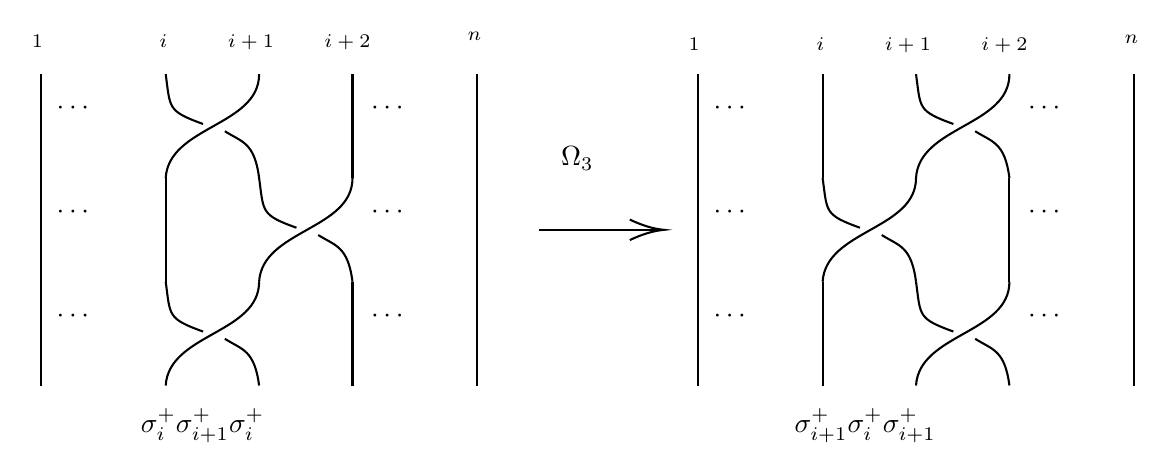
\begin{tikzpicture}[x=0.75pt,y=0.75pt,yscale=-1.5,xscale=1.5]
%uncomment if require: \path (0,335); %set diagram left start at 0, and has height of 335

%Straight Lines [id:da6051419366022395] 
\draw    (130,93.33) -- (130,126.67) ;
%Curve Lines [id:da9988810326669739] 
\draw    (230,93.33) .. controls (230,110) and (201,110) .. (200,126.67) ;
%Curve Lines [id:da22799961222723653] 
\draw    (200,93.33) .. controls (201.5,104.33) and (200.5,105.17) .. (212,109.33) ;
%Curve Lines [id:da1490781175691419] 
\draw    (219,111.67) .. controls (224.5,115.17) and (228.5,115.17) .. (230,126.67) ;
%Straight Lines [id:da8207937248086156] 
\draw    (170,93.33) -- (170,126.67) ;
%Straight Lines [id:da048365350972087495] 
\draw    (270,93.33) -- (270,126.67) ;
%Straight Lines [id:da783175719816261] 
\draw    (130,60) -- (130,93.33) ;
%Curve Lines [id:da21948128892783714] 
\draw    (200,60) .. controls (200,76.67) and (171,76.67) .. (170,93.33) ;
%Curve Lines [id:da11000036284050341] 
\draw    (170,60) .. controls (171.5,71) and (170.5,71.83) .. (182,76) ;
%Curve Lines [id:da2016637435430727] 
\draw    (189,78.33) .. controls (194.5,81.83) and (198.5,81.83) .. (200,93.33) ;
%Straight Lines [id:da03184093892635387] 
\draw    (230,60) -- (230,93.33) ;
%Straight Lines [id:da8580736965744533] 
\draw    (270,60) -- (270,93.33) ;
%Straight Lines [id:da3240339948692498] 
\draw    (130,126.67) -- (130,160) ;
%Curve Lines [id:da15803163782768093] 
\draw    (200,126.67) .. controls (200,143.33) and (171,143.33) .. (170,160) ;
%Curve Lines [id:da6791919280524208] 
\draw    (170,126.67) .. controls (171.5,137.67) and (170.5,138.5) .. (182,142.67) ;
%Curve Lines [id:da9636959373597402] 
\draw    (189,145) .. controls (194.5,148.5) and (198.5,148.5) .. (200,160) ;
%Straight Lines [id:da7737137812536472] 
\draw    (230,126.67) -- (230,160) ;
%Straight Lines [id:da7868366212512278] 
\draw    (270,126.67) -- (270,160) ;
%Straight Lines [id:da9117606281933235] 
\draw    (341,60) -- (341,93.33) ;
%Curve Lines [id:da4617900422359481] 
\draw    (441,60) .. controls (441,76.67) and (412,76.67) .. (411,93.33) ;
%Curve Lines [id:da7919077081110307] 
\draw    (411,60) .. controls (412.5,71) and (411.5,71.83) .. (423,76) ;
%Curve Lines [id:da556973599872705] 
\draw    (430,78.33) .. controls (435.5,81.83) and (439.5,81.83) .. (441,93.33) ;
%Straight Lines [id:da7614386709213076] 
\draw    (381,60) -- (381,93.33) ;
%Straight Lines [id:da03345456947894776] 
\draw    (481,60) -- (481,93.33) ;
%Straight Lines [id:da26200967481729853] 
\draw    (341,93.33) -- (341,126.67) ;
%Curve Lines [id:da09553132514781482] 
\draw    (411,93.33) .. controls (411,110) and (382,110) .. (381,126.67) ;
%Curve Lines [id:da2563544636504017] 
\draw    (381,93.33) .. controls (382.5,104.33) and (381.5,105.17) .. (393,109.33) ;
%Curve Lines [id:da13193755972733046] 
\draw    (400,111.67) .. controls (405.5,115.17) and (409.5,115.17) .. (411,126.67) ;
%Straight Lines [id:da9316135114510464] 
\draw    (441,93.33) -- (441,126.67) ;
%Straight Lines [id:da11527130856596324] 
\draw    (481,93.33) -- (481,126.67) ;
%Straight Lines [id:da3239224345124351] 
\draw    (341,126.67) -- (341,160) ;
%Curve Lines [id:da6738308771610565] 
\draw    (441,126.67) .. controls (441,143.33) and (412,143.33) .. (411,160) ;
%Curve Lines [id:da8633246586798422] 
\draw    (411,126.67) .. controls (412.5,137.67) and (411.5,138.5) .. (423,142.67) ;
%Curve Lines [id:da5645812605701747] 
\draw    (430,145) .. controls (435.5,148.5) and (439.5,148.5) .. (441,160) ;
%Straight Lines [id:da31368590787885864] 
\draw    (381,126.67) -- (381,160) ;
%Straight Lines [id:da4310704090732771] 
\draw    (481,126.67) -- (481,160) ;
%Straight Lines [id:da3326166111695229] 
\draw    (290,110) -- (328,110) ;
\draw [shift={(330,110)}, rotate = 180] [color={rgb, 255:red, 0; green, 0; blue, 0 }  ][line width=0.75]    (10.93,-3.29) .. controls (6.95,-1.4) and (3.31,-0.3) .. (0,0) .. controls (3.31,0.3) and (6.95,1.4) .. (10.93,3.29)   ;

% Text Node
\draw (134,101.4) node [anchor=north west][inner sep=0.75pt]    {$\cdots $};
% Text Node
\draw (235,101.4) node [anchor=north west][inner sep=0.75pt]    {$\cdots $};
% Text Node
\draw (134,68.07) node [anchor=north west][inner sep=0.75pt]    {$\cdots $};
% Text Node
\draw (235,68.07) node [anchor=north west][inner sep=0.75pt]    {$\cdots $};
% Text Node
\draw (134,134.73) node [anchor=north west][inner sep=0.75pt]    {$\cdots $};
% Text Node
\draw (235,134.73) node [anchor=north west][inner sep=0.75pt]    {$\cdots $};
% Text Node
\draw (345,68.07) node [anchor=north west][inner sep=0.75pt]    {$\cdots $};
% Text Node
\draw (446,68.07) node [anchor=north west][inner sep=0.75pt]    {$\cdots $};
% Text Node
\draw (345,101.4) node [anchor=north west][inner sep=0.75pt]    {$\cdots $};
% Text Node
\draw (446,101.4) node [anchor=north west][inner sep=0.75pt]    {$\cdots $};
% Text Node
\draw (345,134.73) node [anchor=north west][inner sep=0.75pt]    {$\cdots $};
% Text Node
\draw (446,134.73) node [anchor=north west][inner sep=0.75pt]    {$\cdots $};
% Text Node
\draw (126,46.4) node [anchor=north west][inner sep=0.75pt]  [font=\scriptsize]  {$1$};
% Text Node
\draw (167,46.4) node [anchor=north west][inner sep=0.75pt]  [font=\scriptsize]  {$i$};
% Text Node
\draw (189,46.4) node [anchor=north west][inner sep=0.75pt]  [font=\scriptsize]  {$i+1$};
% Text Node
\draw (220,46.4) node [anchor=north west][inner sep=0.75pt]  [font=\scriptsize]  {$i+2$};
% Text Node
\draw (266,45.4) node [anchor=north west][inner sep=0.75pt]  [font=\scriptsize]  {$n$};
% Text Node
\draw (337,47.4) node [anchor=north west][inner sep=0.75pt]  [font=\scriptsize]  {$1$};
% Text Node
\draw (378,47.4) node [anchor=north west][inner sep=0.75pt]  [font=\scriptsize]  {$i$};
% Text Node
\draw (400,47.4) node [anchor=north west][inner sep=0.75pt]  [font=\scriptsize]  {$i+1$};
% Text Node
\draw (431,47.4) node [anchor=north west][inner sep=0.75pt]  [font=\scriptsize]  {$i+2$};
% Text Node
\draw (477,46.4) node [anchor=north west][inner sep=0.75pt]  [font=\scriptsize]  {$n$};
% Text Node
\draw (296,82.4) node [anchor=north west][inner sep=0.75pt]    {$\Omega _{3}$};
% Text Node
\draw (161,166.4) node [anchor=north west][inner sep=0.75pt]    {$\sigma _{i}^{+} \sigma _{i+1}^{+} \sigma _{i}^{+}$};
% Text Node
\draw (371,166.4) node [anchor=north west][inner sep=0.75pt]    {$\sigma _{i+1}^{+} \sigma _{i}^{+} \sigma _{i+1}^{+}$};


\end{tikzpicture}
    \end{center}
Con todo esto estamos preparados para probar nuestro primer resultado de equivalencia
\begin{theorem}
    Para $\varepsilon=\pm,$ existe un unico homomorfismo $\varphi_{\varepsilon}:B_n\to\mathcal{B}_n$ tal que \\$\varphi_{\varepsilon}(\sigma_i)=\sigma_i^{\varepsilon}$ para todo $i=1,\ldots n-1.$ Ademas el homorfismo $\varphi_\varepsilon$ resulta ser un isormorfismo. 
\end{theorem}
\begin{proof}
    Debido a la similitud de ambas pruebas solo haremos el caso $\varepsilon=+$. Por la proposición 3.2 y el Lema \ref{homoexis} existe un único homomorfismo $\varPhi_{+}$ que cumple lo deseado. Luego por la prueba de la proposición 3.1 sabemos que los $\sigma_i^+$ generan $\mathcal{B}_n$ asi el homomorfismo es sobreyectivo. Para la inyectividad sea $\beta\in \mathcal{B}_n$ representada por su diagrama de trenzas $D$ con la representación presentada en la proposición 3.1, es decir
     $$\beta=\beta(D)=\sigma_{i_1}^{\varepsilon_1}\dots\sigma_{i_k}^{\varepsilon_k},$$
     y definamos $\psi:\mathcal{B}_n\to B_n$ tal que
     $$\psi(D)=(\sigma_{i_1})^{\varepsilon_1}\dots(\sigma_{i_k})^{\varepsilon_k}.$$
     Donde las potencias $\varepsilon_j=\pm$ significan en $B_n$ el tomar el elemento usual o su inverso. Note que si $\psi$ esta bien definido entonces como función por construcción $\psi\circ \varphi_{+}=id_{B_n}$, luego como mostramos la existencia de una inversa a izquierda, $\varphi_{+}$ es inyectiva y por tanto un isomorfismo. Mostremos que la imagen $\psi(D)$ depende unicamente de $\beta$. Por el teorema 2.15 basta ver que la imagen se preserva bajo secuencias finitas de isotopias de $D$ y movimientos de $\Omega_2$ y $\Omega_3$ (el caso de los inversos es equivalente). Primero observe que las isotopias que preservan el orden de los puntos de corte dado por la expansión no alteran $D$ y por tanto $\psi(D)$ no se altera. Si una isotopia cambia el orden de dos puntos de corte, eso es equivalente a cambiar en la expresión $\sigma_i^{\varepsilon_i}\sigma_j^{\varepsilon_j}$ por $\sigma_j^{\varepsilon_j}\sigma_i^{\varepsilon_i}$ con $|i-j|\geq 2$. Bajo $\psi$ note que estas dos expresiones son iguales en $B_n$ por la primera relación del grupo de trenzas.\\

     Para $\Omega_2$ esto lo que hace es que inserta un $\sigma_i^+\sigma_i^-$ o $\sigma_i^-\sigma_i^+$ a la expresión de $D$, luego al enviarla por $\psi$ al ser inversos queda la misma $\psi(D).$ El movimiento $\Omega_3$ en la expresión de $D$ reemplaza una secuencia $\sigma_i^+\sigma_{i+1}^+\sigma_i^{+}$ por $\sigma_{i+1}^+\sigma_{i}^+\sigma_{i+1}^{+}$, pero en $\psi(D)$ estas dos son iguales en $B_n$ por la segunda relación de trenzas. Así concluimos lo deseado.

\end{proof}

Esto nos permite intercambiar libremente entre las trenzas geométricas y algebraicas, por lo que de ahora en adelante nos referiremos a cualquier elemento en $B_n$ como \textit{trenzas en n cuerdas}, esto nos permite hacer algunas observaciones de $B_n$ desde la vista geometrica, que solo desde el álgebra habría sido difícil de probar
\begin{corollary}
    La inclusión $i:B_n\to B_{n+1}$ es inyectiva para todo $n.$
\end{corollary}
\begin{proof}
    Geometricamente la inclusión es tomar una trenza en $n$ cuerdas y añadir una cuerda extra a la derecha del diagrama que no interactué con las demás, resultando en una trenza en $n+1$ cuerdas. Así dadas $b_1$ y $b_2$ trenzas geometricas tales que $i(b_1)$ y $i(b_2)$ isotopicas, como ambas trenzas tienen la cuerda $n+1$ fija, si las restringimos a las primeras $n$ cuerdas obtenemos una isotopia de $b_1$ y $b_2$, así $i$ es inyectiva.
    
\end{proof}